\documentclass[sigconf, 9pt]{acmart}

\usepackage{booktabs} % For formal tables

\usepackage{graphicx,epsfig,color,endnotes,alltt}
\usepackage{caption}
\DeclareCaptionType{copyrightbox}
%\usepackage{subcaption}
\usepackage{comment}
\usepackage{keyval}
\usepackage{subfig}
\usepackage{url}
\usepackage{balance}
\usepackage [ruled,linesnumbered] {algorithm2e}  \usepackage[noend]{algorithmic}
\usepackage{fancyvrb}
\usepackage[noindent, nolineno]{lgrind}
\usepackage{epstopdf}
\usepackage{array}
\usepackage{multirow}
\usepackage{amsmath}
\usepackage{bm}
\usepackage{slashbox}

\usepackage{xcolor}
\usepackage{listings}
\definecolor{dkgreen}{rgb}{0,0.6,0}
\definecolor{gray}{rgb}{0.5,0.5,0.5}
\definecolor{mauve}{rgb}{0.58,0,0.82}
\lstset{basicstyle=\ttfamily\footnotesize,
        breaklines=true,
        frame=single, 
        language=C++,  %lauguage of code
        otherkeywords={*, hello}, %extra keywords
        escapeinside={\%*}{*)},        
        morecomment=[l][\color{gray}]{//},
        keywordstyle=\color{blue},
        stringstyle=\color{mauve}
        commentstyle=\color{dkgreen}, 
        moredelim=**[is][\color{red}]{@}{@},
%        moredelim=**[is][\color{blue}]{#}{#}
       }

\usepackage[titletoc,title]{appendix}


\setcopyright{rightsretained}

% Commands added by Juan 
\definecolor{dgreen}{rgb}{0.00, 0.75, 0.00}
\newcommand{\jgl}[1]{[{\color{dgreen}JGL: #1}]}
\newcommand{\juan}[1]{{\color{dgreen}#1}}

% DOI
\acmDOI{}%10.475/123_4}

% ISBN
\acmISBN{}%123-4567-24-567/08/06}

%Conference
\acmConference[DAC'19]{ACM conference}{June 2019}{Las Vegas, USA} 
\acmYear{2019}
\copyrightyear{2019}

\acmPrice{15.00}

\graphicspath{{./figure/}}


\begin{document}
	
%\title{Understanding and Optimizing OpenCL Kernels on FPGAs}
%\title{Go-beyond OpenCL or Not: Deciding Performance Upper Bound of OpenCL Kernel on FPGAs}
\title{Go-beyond OpenCL or Not: Optimizing OpenCL Kernel on FPGAs}

\begin{abstract}
%Hello abstract.
For a broad range of applications, FPGA architecture allows a massive bit-level parallelism to be exploited to achieve high performance and energy efficiency. Therefore, the parallel nature of FPGA inherently matches the parallel programming language, e.g., OpenCL. For example, FPGA vendors such as Intel have released OpenCL SDK for FPGAs so that FPGA programmer can now leverage OpenCL to program FPGA, instead of tedious, time-consuming and error-prone register transfer level (RTL). %which impedes the widespread adoption of FPGAs by software programmers. 
Accordingly, a wealth of literature have explored multiple optimization methods (e.g., loop unrolling) to accelerate conventional OpenCL (i.e., NDRange kernel) on FPGAs. 
%Despite the preliminary success of OpenCL on FPGAs, we have still identified that . The main difference comes in two flavours: single work-item kernel and OpenCL channel, which are referred to two go-beyond OpenCL features in this paper. 
However, conventional OpenCL cannot always represent FPGA architecture in an efficient manner, since OpenCL is originally designed for GPUs. Accordingly, Intel OpenCL SDK provides two go-beyond OpenCL features (single work-item kernel and OpenCL channel) to better utilize FPGA resources. However, how to leverage go-beyond OpenCL features is still unclear to the conventional OpenCL programmer.  
In this paper, we reduce the problem (go-beyond OpenCL features or not) to the problem of bridging the gap between three typical OpenCL patterns and four execution models (aware of go-beyond OpenCL features). Essentially, the OpenCL programmer can easily determine whether to employ go-beyond OpenCL features, based on whether the interested OpenCL code contains any OpenCL patterns or not. Experimental result shows that, 1)choosing the suitable execution model can lead to up to three orders of magnitude performance speedup over the most unsuitable execution model; 2)we can determine the right execution model via three OpenCL patterns plus an analytical model. Therefore, we argue the execution model should be considered as the first step to decide, as it decides the potential of other optimization combinations can reach. 
%reduce the problem explicitly .

%This paper is orthogonal to the existing literature.
%As a complementary guideline for the existing optimization efforts. But

%the conventional OpenCL programmer .the existing work does not take into account go-beyond OpenCL features (i.e., ). In other words, 

%The parallel programming languages, e.g., OpenCL, are based on BSP (Bulk Synchronous Parallel) model and are widely adopted by GPUs, which feature a massive number of cores for the computation task. Due to the fact that , it is a natural attempt to use the existing parallel programming languages to program FPGA. Additionally, parallel programming language delivers increased programmability and lower learning curve with respect to RTL. For instance, Intel has launched one OpenCL SDK to program FPGAs~\cite{altera_optimization}. Plenty of research work~\cite{flexcl_tc18, opencl_compiler_ERSA12, fpga_opencl_model_hpca16} are aim at optimizing the \emph{conventional OpenCL} kernels on FPGAs, where the conventional OpenCL kernel is the NDRange kernel which employs a multi-thread approach to explore the thread-level parallelism to accelerate the computing task. 

%1, OpenCL on GPUs is popular, it is natural to try OpenCL on FPGAs 


%Somewhere in the introduction, it is necessary to talk about the characteristics of the GPU OpenCL codes that are going to be ported to FPGA in this work. In Chai \cite{gomez2017chai}, there are benchmarks that use inter-kernel communication (e.g., CEDD) and multi-pass schemes (e.g., BFS, SSSP). These two are typical techniques in GPU programming. In Chai, there is also extensive use of atomic operations. In the past, GPU programmers avoided atomic operations \cite{nasre2013} because they had high overhead. However, in recent GPU generations (e.g., NVIDIA Kepler, Maxwell, Pascal) the hardware has greatly improved. They provide improved programmability that GPU programmers nowadays leverage.


\end{abstract}




\maketitle

\vspace{-1ex}
\section{Introduction}

The parallel programming languages, e.g., OpenCL, are based on BSP (Bulk Synchronous Parallel) model and are widely adopted by GPUs, which features a massive number of cores for the computation task. 
Due to the fact that FPGA is embarrassingly parallel, it is a natural attempt to use the existing parallel programming languages to program FPGA \jgl{Also because of increased programmability and lower learning curve with respect to RTL}. For instance, Intel has launched one OpenCL SDK to program FPGAs~\cite{altera_optimization}. Plenty of research work~\cite{flexcl_tc18, opencl_compiler_ERSA12, fpga_opencl_model_hpca16} are aim at optimizing the \emph{conventional OpenCL} kernels on FPGAs, where the conventional OpenCL kernel is the NDRange kernel which employs a multi-thread approach to explore the thread-level parallelism to accelerate the computing task. 
%The optimization process is vital to achieve good performance on FPGAs, since the performance difference between proper and improper optimizations can be significant. For example, [X] shows that the optimal combination of optimization methods can provide two orders of magnitude better performance than the baseline without optimization. 

\jgl{I think an interesting motivation for this work can be achieving performance portability across different types of accelerators (i.e., GPU to FPGA). In this regard, a paper to cite is \cite{chang2017collaborative}.}

\jgl{Somewhere in the introduction, it is necessary to talk about the characteristics of the GPU OpenCL codes that are going to be ported to FPGA in this work. In Chai \cite{gomez2017chai}, there are benchmarks that use inter-kernel communication (e.g., CEDD) and multi-pass schemes (e.g., BFS, SSSP). These two are typical techniques in GPU programming. In Chai, there is also extensive use of atomic operations. In the past, GPU programmers avoided atomic operations \cite{nasre2013} because they had high overhead. However, in recent GPU generations (e.g., NVIDIA Kepler, Maxwell, Pascal) the hardware has greatly improved. They provide improved programmability that GPU programmers nowadays leverage.}

Despite the preliminary success from directly adopting conventional OpenCL programs on FPGAs, we still identify a significant gap from achieving the near-to-optimal performance on FPGAs due to the factor that the conventional OpenCL kernel is not able to fully utilize two distinguished architectural features of FPGAs \jgl{Any related work that has compared the performance of optimized RTL with OpenCL?}. We refer this kind of direction as a go-beyond OpenCL on FPGAs. %We discuss the features in two dimensions. %the architecture of FPGAs is significantly different from that of GPUs

\vspace{0.3em}
\noindent
{\bf F1: Single Work-Item (SWI) Kernel. } Intel OpenCL SDK provides a new programming model for FPGAs: \emph{single work-item kernel}. It relies on the off-line compiler to explore the pipelined parallelism at the compilation time. Therefore, it only contains only one work item to do the computation, indicating significantly different from data-parallel programming model of conventional OpenCL kernel. %The single work-item execution pattern more closely matches the traditional deep-pipeline approach of programming FPGAs.
%First, the external memory bandwidth on FPGAs is critically less than that on GPUs. This means that memory bandwidth on FPGAs can much easier become the performance bottleneck.  

\vspace{0.3em}
\noindent
{\bf F2: Direct Kernel-to-Kernel Communication. }The communication between two kernels can be done via a Fifo (i.e., OpenCL channel) on FPGAs, not via memory subsystem like GPUs. It can potentially reduce memory traffic and achieve more parallelism by concurrently executing multiple OpenCL kernels on FPGAs. 
%OpenCL programs are originally designed for GPUs

Actually, several research work~\cite{partition_fpl15, gzip_iwocl14} have already employed the above two techniques to significantly accelerate a broad range of OpenCL applications. For instance, the performance of database partitioning~\cite{partition_fpl15} is improved by 10.7 times, indicating a great potential of go-beyond kernel on FPGAs. Together with the optimization methods from conventional OpenCL kernel, a huge design space needs to be explored to determine the optimal (or near-to-optimal) optimization combination on FPGAs. 
Unfortunately, there is no comprehensive study to guide how to optimize the OpenCL kernels on FPGAs, especially about go-beyond OpenCL kernels. Therefore, the burden of choosing the right OpenCL optimization methods still falls on the users without any rule-of-thumb guidelines. %In this paper, we try to bridge the gap between application and OpenCL execution pattern. In particular, 
%a comprehensive study, which can  is still lacking.
In this paper, we try to answer the following question: {\em Can we narrow the gap between conventional OpenCL programmer and performance potential of FPGAs?}
%\vspace{-0.2em}
%\begin{center}
%	{\em Can we bridge the gap between conventional OpenCL programmer and high performance on FPGAs?}
%\end{center}
%\vspace{-0.2em}

%As a start, we try to bridge the gap between OpenCL patterns and execution models.
In this paper, we make the following contributions to narrow the gap for the conventional OpenCL programmer by connecting three common OpenCL patterns and four high-level execution models.

\jgl{To me, the most significant contribution of this work can be providing some guidelines on how to transform optimized GPU OpenCL code into optimized FPGA OpenCL.} 

\vspace{0.4em}
\noindent
{\bf C1: Three OpenCL Patterns on FPGAs (Section~\ref{sec_patterns}). }We identify three popular patterns from OpenCL kernels: atomic operation, multi-pass scheme and kernel-to-kernel communication, which are worth to be heavily revisited on FPGAs, since their performance can be significantly improved with the help of go-beyond-OpenCL features enabled by FPGAs. These patterns are well understood by the conventional OpenCL programmers such that they can easily identify the potentials of their original OpenCL program when mapping them onto FPGAs. %Besides,  can easily understand these patterns. %the architecture of FPGAs is significantly different from that of GPUs. In particular, 

\vspace{0.4em}
\noindent
{\bf C2: Four High-level Execution Models on FPGAs (Section~\ref{sec_execution_models}). }We identify four high-level OpenCL execution models: NDRange, SWI, NDRange+Channel and SWI+Channel, which serve as main guidelines on how to optimize the OpenCL program on FPGAs. Choosing the right high-level execution model is vital for OpenCL program to achieve excellent performance on FPGAs. We also generally compare the characteristics of four execution models, which are aware of the advanced features of go-beyond OpenCL kernel. 

%\vspace{0.4em}
%\noindent
%{\bf C3. Bridge the Gap between Patterns and Execution Models. }We identify three OpenCL patterns which show great opportunity to...
%
%Bridge the gap between OpenCL programmer and FPGAs. In particular, we provide a OpenCL-programmer-understandable approach 
\vspace{0.4em}
\noindent
{\bf C3. Intensive Experiment to Verify Our Observation (Section~\ref{sec_experiment}). }We implement and optimize 11 OpenCL applications on a Terasic\textquoteright s DE5A-Net Arria 10 FPGA board. Actually, we try our best to implement all the execution models\footnote{For few applications, it is impossible to implement few execution models.}, each of which contains multiple optimization combinations, for each application. Based on the experimental result, we can make two observations. First, different high-level execution model leads to up to two orders of magnitude performance difference\footnote{Based on our five years' experience on OpenCL-based FPGAs, we are pretty sure that our implementation have typically reached the near-to-optimal performance for each execution model. We will make all the related source code open-sourced. }, as shown in Figure~\ref{XXX}. Second, we identify a obvious connection between three proposed OpenCL channels and four high-level execution models. %We try to show the potential of different execution models by quantitatively analyze the performance difference. 


\vspace{1em}
\noindent
{\bf Future Directions and Limitation.} 
To the best of our knowledge, this paper is the first attempt to narrow the gap between conventional OpenCL programmer and FPGAs, and we believe it opens a few exciting research directions which aim at closing the gap so that it will attract more and more people to devote to FPGA acceleration. One interesting future direction is to provide an end-to-end performance analytical model to predict the performance of each execution model. Unfortunately, only the NDRange kernel is well studied in terms of the analytical model~\cite{fpga_opencl_model_hpca16, flexcl_tc18}. 
Another interesting future direction is to design an automatic optimization process for each execution model with the help of performance analytical model. As such, more and more people without any FPGA background can take advantage of computing power of FPGAs. 


The limitation is that we manually try plenty of optimization combinations for each execution model. %Based on our five years' experience on OpenCL-based FPGAs, we are pretty sure that our implementation have typically reached the near-to-optimal performance for each execution model. 

%Deciding the right execution pattern is rule-of-thumb to determine the performance of  




%Third, where communication among cores is done via memory subsystem, e.g., external memory. In particular, each core writes its result to the memory subsystem and then synchronize to make sure the core can see the latest result from other cores. The underlying reason is that no communication channel exists between any two cores. This execution pattern works well on GPUs due to its powerful memory subsystem



%in this paper, we explore the design space of accelerating OpenCL programs on FPGAs, especially focusing on the go-beyond OpenCL part. In particular, 

%Towards a comprehensive 


\vspace{-1ex}
\section{Background}
%@Jiantong, you can fill this section, following my paper's style. 

\subsection{Traditional OpenCL Programming Model}

\subsubsection{OpenCL Concepts} 
%work item, work group, et at. 

OpenCL is an open parallel programming language for heterogeneous computing environments. It aims for a host-accelerator model of program execution, where a host processor runs control-intensive task and offloads computation-intensive code (i.e., \emph{kernel}) onto an external accelerator.

Recently, Altera provides the OpenCL SDK to abstract the hardware complexities from the traditional FPGA design. The Altera's SDK can translate the high-level OpenCL description to low-level hardware implementation by creating the circuits for each operation of the kernel and interconnect them together to achieve the whole data path.

From the perspective of OpenCL, the FPGA memory hierarchy  contains three layers. First, the \emph{global memory} with high latency and low bandwidth which often refers to the DDRs of the FPGA board. Second, the \emph{local memory} utilizes on-chip low-latency and high-bandwidth BRAMs, and it has four banks in general. Third, the \emph{private memory}, storing the variables or small arrays for each work-item, is constructed using completely-parallel registers. Compared to CPU/GPU, the private memory is rather plentiful in FPGA.

Different from viewing FPGAs as pure hardware resources like LUTs, DSP blocks and memory blocks, the OpenCL SDK regards the FPGA as a large-scale parallel architecture. Most commonly, OpenCL partitions a problem into equally loaded chunks of work, i.e., \emph{work-item}, which represent the basic unit of execution. A set of work-items are organized into a \emph{work-group} and multiple work-groups are combined to form a three-dimensional index space called \emph{NDRange}. \emph{NDRange kernel} is the default OpenCL kernel model which achieves the pipelined parallelism across multiple work-items. We can configure multiple kernel pipelines, i.e., Compute Units (CUs) for the NDRange kernel. Then each CU executes the OpenCL program in a pipelined fashion. Although NDRange execution pattern is the most common pattern of using accelerators with OpenCL, it is not mandatory. Actually, in many cases, single work-item kernels are employed as a preferred execution pattern in Altera's OpenCL implementation as explained below.


\subsubsection{Main Optimization Methods}
We introduce three main optimization methods, which are widely adopted by normal and go-beyond OpenCL kernels. We refer the reader to the related work~\cite{fpga_opencl_model_hpca16} for more optimization methods on FPGAs. 

{\bf Shared Memory. } Each CU has its own local memory, which is shared by all the work-items assigned to the CU, while all CUs share a global memory. The on-chip local memory is low-latency and high-throughput compared to global memory. Thus, the local memory can be employed to reduce the number of global memory accesses.

{\bf Loop Unrolling. } If there are a large number of loop iterations in the kernel pipeline, the loop iterations could potentially be the critical path of the kernel pipeline. Unrolling the loop can increase the pipeline throughput at the expense of more hardware resources consumption. And it may have a side-product benefit on FPGAs. The load/store operations can coalesce so that the number of global memory accesses is reduced.

{\bf Multiple Compute Units. } If the hardware resource is sufficient on the FPGA, the kernel pipeline can be replicated to generate multiple CUs for each kernel and the inner hardware scheduler automatically dispatches work-groups to available CUs. Kernel pipeline replication can achieve higher throughput at the expense of increasing hardware resource utilization, which often leads to a lower FPGA operating frequency than that of one CU. It means that two CUs cannot always double the performance. Another issue is that the global memory load/store operations from multiple CUs compete for the global memory bandwidth and the total number of global memory operations remains unchanged.


\subsection{Go-beyond OpenCL on FPGAs}

\subsubsection{Single Work-Item Kernel} 

In addition to the standard NDRange kernel model, Altera OpenCL SDK also provides a \emph{single work-item kernel}  model. It follows a sequential model like C programming, thus executes the kernel on only one CU that contains only one work-item. In the single work-item execution pattern, the parallelism is implicit, and the OpenCL SDK will instead determine pipelined parallelism at the compilation time based on the dependency. The single work-item execution pattern more closely matches the traditional deep-pipeline approach of programming FPGAs.


\subsubsection{OpenCL Channel}

Altera OpenCL SDK provides the \emph{OpenCL channel} feature, which can be used to pass data between two OpenCL kernels (either NDRange or single work-item) and synchronize the kernels with high efficiency and low latency. In the conventional OpenCL implementation, the communication between two kernels is performed via global memory. However, global memory bandwidth could potentially be a performance bottleneck for the kernels. In contrast, the implementation of channels decouples kernel execution from the host processor, allowing the kernels to communicate directly with each other via on-chip FIFO buffers.

The OpenCL channel has two types: blocking channel and nonblocking channel. The write/read operation to blocking channel will not return if the operation does not successfully commit, while the write/read operation to nonblocking channel will return even when the operation does not successfully commit.

%The second paragraph has not been modified.







\vspace{-1ex}
\section{Design Overview}
In this section, we illustrate how the next three sections organized. 
In Section~\ref{sec_patterns}, we identify three typical OpenCL patterns, which are well understood by the conventional OpenCL programmer with GPUs.
In Section~\ref{sec_execution_models}, we generally analyze the characteristics of four OpenCL execution models, which takes into account the go-beyond OpenCL features enabled on FPGAs.
In Section~\ref{sec_bridge_gap}, we explicitly bridge the gap between OpenCL patterns and execution models on FPGAs. Choosing the right execution model determines the performance upper bound of the interested OpenCL application can reach. %can deliver an order of magnitude performance difference. 
\vspace{-1ex}
\section{Three OpenCL Patterns}%: Issue and Potential
\label{sec_patterns}
%The conventional OpenCL is originally designed for GPUs which have super powerful memory subsystem, 
When migrating conventional OpenCL programs, which is originally designed for GPUs, we identify three OpenCL patterns which can be significantly improved: atomic operation, multi-pass scheme and communication approach. In the following, we analyze the issue and potential optimization direction of each pattern on FPGAs.

\vspace{-1ex}
\subsection{Atomic Operation (AO)}
For NDRange OpenCL, the atomic operation is required to guarantee the consistence of OpenCL kernel, when multiple work items try to update the same memory location~\cite{opencl_spec, atomic_fpga16}. It provides the improved programmability that GPU programmers nowadays leverage, since the hardware for the atomic operation has greatly improved in recent GPU generations (e.g., NVIDIA Kepler, Maxwell, Pascal).
Take as an example the simplified histogram, whose main body is illustrated in Listing~\ref{list_atomic_histo}. %, style=base

%\begin{lstlisting}[caption={Atomic-based histogram},label={list_atomic_histo},captionpos=b]
\begin{lstlisting}[caption={Atomic-based histogram},label={list_atomic_histo},captionpos=b]
int tid = get_global_id(0);//global work item
int d   = data[tid];       //fetch the data from memory
int h_d = hash(d);         //compute the hash index
atomic_add(&@hist@[h_d],1);  //atomically add to hist
\end{lstlisting}

%@jiang, add one example here.

{\bf Issues on FPGAs. }We have identified three issues regarding atomic operation on FPGAs. First, the mechanism of atomic operation is relatively complex, so massive FPGA resources are required to implement it, leading to a noticeable resource overhead on FPGAs. %and then this issue on FPGAs is much worse on ASICs. 
Second, with atomic operation in our OpenCL kernel, all the memory transactions, including both atomic and normal memory transactions, have to enter the atomic module to guarantee the correct execution, as atomic and normal memory transactions from OpenCL kernel can reference the same memory location. Therefore, each memory transaction has a longer memory access latency, leading to potentially lower memory bandwidth.  
Third, the frequency of OpenCL kernel with atomic operation is slightly lower than that without atomic operation, leading to lower performance. We conclude that the atomic operation is not able to fit well on FPGAs.  % has severe performance issue \jgl{Every access goes through the atomic path even though it is clear that there are no atomic accesses to certain arrays? This is weird, but reminds me that something similar happened in old AMD GPUs}

{\bf Potential on FPGAs. }In order to achieve good performance of OpenCL kernel on FPGAs, one potential direction is to get rid of atomic operation. Fortunately, Intel OpenCL SDK~\cite{altera_optimization} supports a new execution model: SWI kernel. Essentially, it contains only one work item during the kernel execution, so there is no conflict from multiple work items, indicating that no atomic operation is required. Instead, it exploits the pipelined parallelism, not the thread-level parallelism which is widely exploited by GPUs. The previous histogram application is converted into the SWI kernel as shown in Listing~\ref{list_swi_histo}. 

\begin{lstlisting}[caption={SWI-based histogram},label={list_swi_histo},captionpos=b]
for (t=0; t<size; t++) { //for loop instead of work item
  int d   = data[t];     //fetch the data from memory
  int h_d = hash(d);     //compute the hash index
  @hist@[h_d] += 1;        //accumulate to hist
}
\end{lstlisting}


\vspace{-1ex}
\subsection{Multi-Pass Scheme (MPS)}
The multi-pass scheme is widely adopted to leverage a massive amount of cores in CPUs/GPUs to accelerate parallel algorithm, e.g., database operators~\cite{query_gpu_tods09, omnidb_vldb13, query_openCL_fpga_fpl16}. Besides, it can also improve the cache locality on GPUs, e.g., gather/scatter~\cite{gather_scatter_sc07}, so as to increase the overall parallelism at the cost of more memory traffic. Take the simplified parallel prefix sum~\cite{scan_gpu_nvidia07} as an example, we perform the prefix sum on the input array \emph{in} of size \emph{N} and store the output in the array \emph{out}, as illustrated in Listing~\ref{list_parallel_scan}. In Step 1, B work groups (WGs) executes concurrently, each WG performs the prefix sum (kernel \emph{prefix\_sum\_wg}) on its own part of data of starting address \emph{in[N*b/B]} and of length \emph{N/B}. Meanwhile, each WG stores its local sum to \emph{local\_sum}. In Step 2, we employ one WG to compute the prefix sum on \emph{local\_sum} and store to \emph{pre\_bsum}. In Step 3, each WG adds the scalar value \emph{pre\_bsum} to the vector and then produces the final prefix sum. 

% illustrates the B-work-group parallelism. 
\begin{lstlisting}[caption={MPS-based prefix sum},label={list_parallel_scan},captionpos=b]
//Step 1: each WG computes the prefix sum on its own data
#progama parallel in B work groups
for (b = 0, b < B, b++) { 
  local_sum[b] = prefix_sum_wg(@out@[N*b/B],@in@[N*b/B],N/B);
}

//Step 2: one WG computes the prefix sum on "local_sum"
prefix_sum_wg(pre_bsum, local_sum, B);

//Step 3: out@[b*N/B] += pre_bsum[b]
#progama parallel in B work groups
for (b = 0, b < B, b++) {
  vec_add(@out@[b*N/B], @out@[b*N/B], pre_bsum[b], N/B);
}
\end{lstlisting}
%Therefore, the multi-pass scheme, which heavily relies on high memory bandwidth, can still achieve better performance on GPUs than on CPUs, even though it requires multiple times more memory traffic than the original sequential counterpart which may run on a single CPU core. 
%requires multiple passes~\cite{query_gpu_tods09} to finish the computation task, e.g., database scan. In other words,

{\bf Issues on FPGAs. }We observe that the inevitable requirement for the widespread adoption of multi-pass scheme is powerful memory subsystem, as it always requires multiple times more memory traffic to realize the algorithm. It works pretty well on GPUs, whose memory bandwidth is almost an order of magnitude larger than the same-generation CPU or FPGA. For example, the memory bandwidth of Nvidia Tesla P100 GPU is able to reach 732GB/s, while Intel Skylake i9-7980XE CPU has the memory bandwidth of 85GB/s and Xilinx UltraScale+ FPGA board has 48GB/s. We can predict that the multi-pass scheme, whose success heavily relies on high memory bandwidth, would be less popular on FPGAs than on GPUs, since the memory bandwidth of FPGAs is relatively low, e.g., 18GB/s on our tested FPGA board. Therefore, it suffers from its severe performance issue, especially for the memory-bound OpenCL kernel, even though the FPGA can provide massive thread-level parallelism in terms of pipelined parallelism. 

{\bf Potential on FPGAs. } Since Intel OpenCL SDK for FPGAs supports the new single work-item kernel, the OpenCL kernel is allowed to be implemented in a single-pass approach, as illustrated in Listing~\ref{list_swi_scan}. %, without compromising any achievable pipeline parallelism 
Therefore, the memory traffic is reduced to a minimum level (i.e., accessing the array \emph{in/out} once, not twice) just as the single-threaded implementation running on a single CPU core. 
%We can use single-work item execution model: multi-pass approach to approach. %It means that the memory traffic 
\begin{lstlisting}[caption={SWI-based prefix sum},label={list_swi_scan},captionpos=b]
out[0] = 0;
for (t=1; t<n; t++) { //for loop instead of work item
  @out@[t] = @out@[t-1] + @in@[t]; //dependency in out
}
\end{lstlisting}



\vspace{-1ex}
\subsection{Kernel-to-Kernel Communication (KKC)}
On GPUs, the typical communication approach between producer/consumer kernels is done via global memory. In particular, after the producer kernel writes the data to the global memory, the consumer kernel reads the data from global memory, as illustrated in Figure~\ref{fig_without_channel}. It is a common communication approach to exchange information among Stream Processors (SPs) in GPUs, as there is no physical communication path between any two SPs. This communication approach works well on GPUs since GPUs can execute each kernel relatively fast due to its massive thread-level parallelism and powerful memory subsystem. Suppose each OpenCL kernel is fully optimized, the overall performance of producer/consumer kernels is maximized. %Even though more memory traffic is required to 
This communication approaches widely used in accelerating various applications, e.g., database~\cite{query_gpu_tods09, omnidb_vldb13}. 

{\bf Issue on FPGAs. }The memory bandwidth is relatively low on FPGAs, e.g., 18GB/s on our FPGA board, the communication via external memory can be expensive, compared with that on GPUs. 

{\bf Potential on FPGAs. }We can use OpenCL channel via which the producer kernel can directly send data to the consumer kernel at the register level (i.e., FIFO), without any memory traffic involved between the producer and consumer kernels, as illustrated in Figure~\ref{fig_with_channel}. Besides, both kernels, each of which has the dedicated hardware resources to implement, execute concurrently, so not only intra-kernel parallelism (i.e., pipelined) is exploited, but also inter-kernel parallelism (i.e., multiple kernels).  
\begin{figure}
	\centering
	%\hfill
	\subfloat[Without channel]{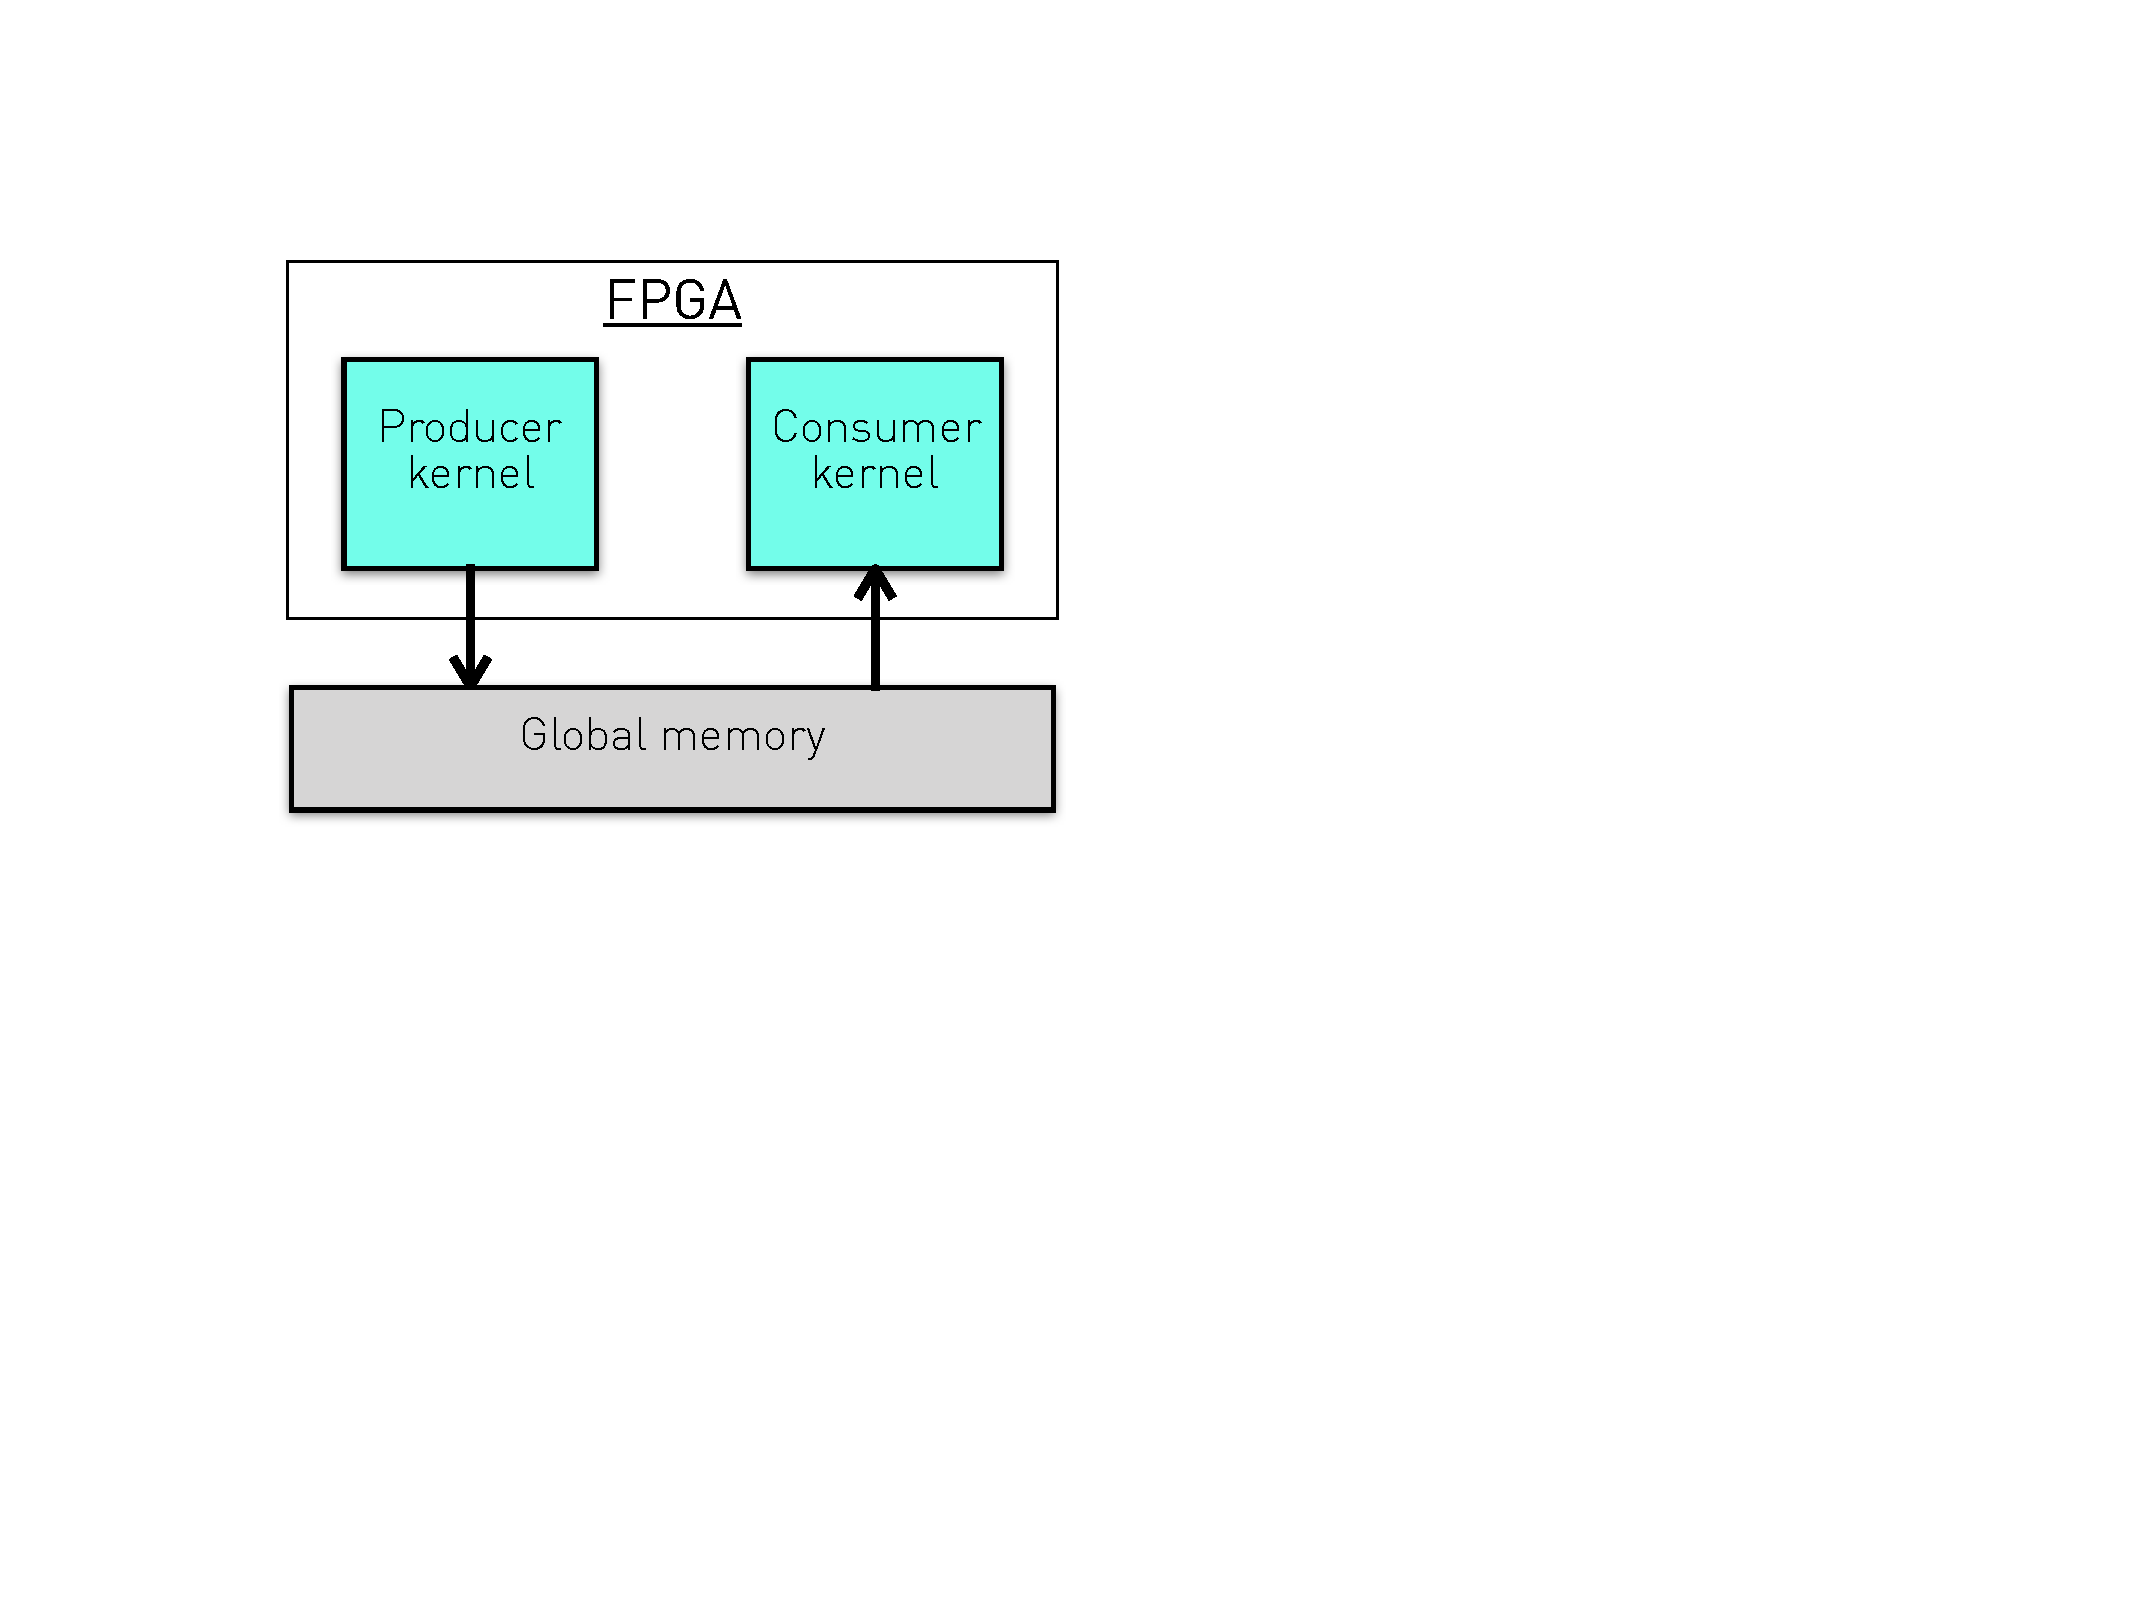
\includegraphics[width=1.415in]{without_channel1.pdf} 
		\label{fig_without_channel}} 
	\subfloat[With channel]{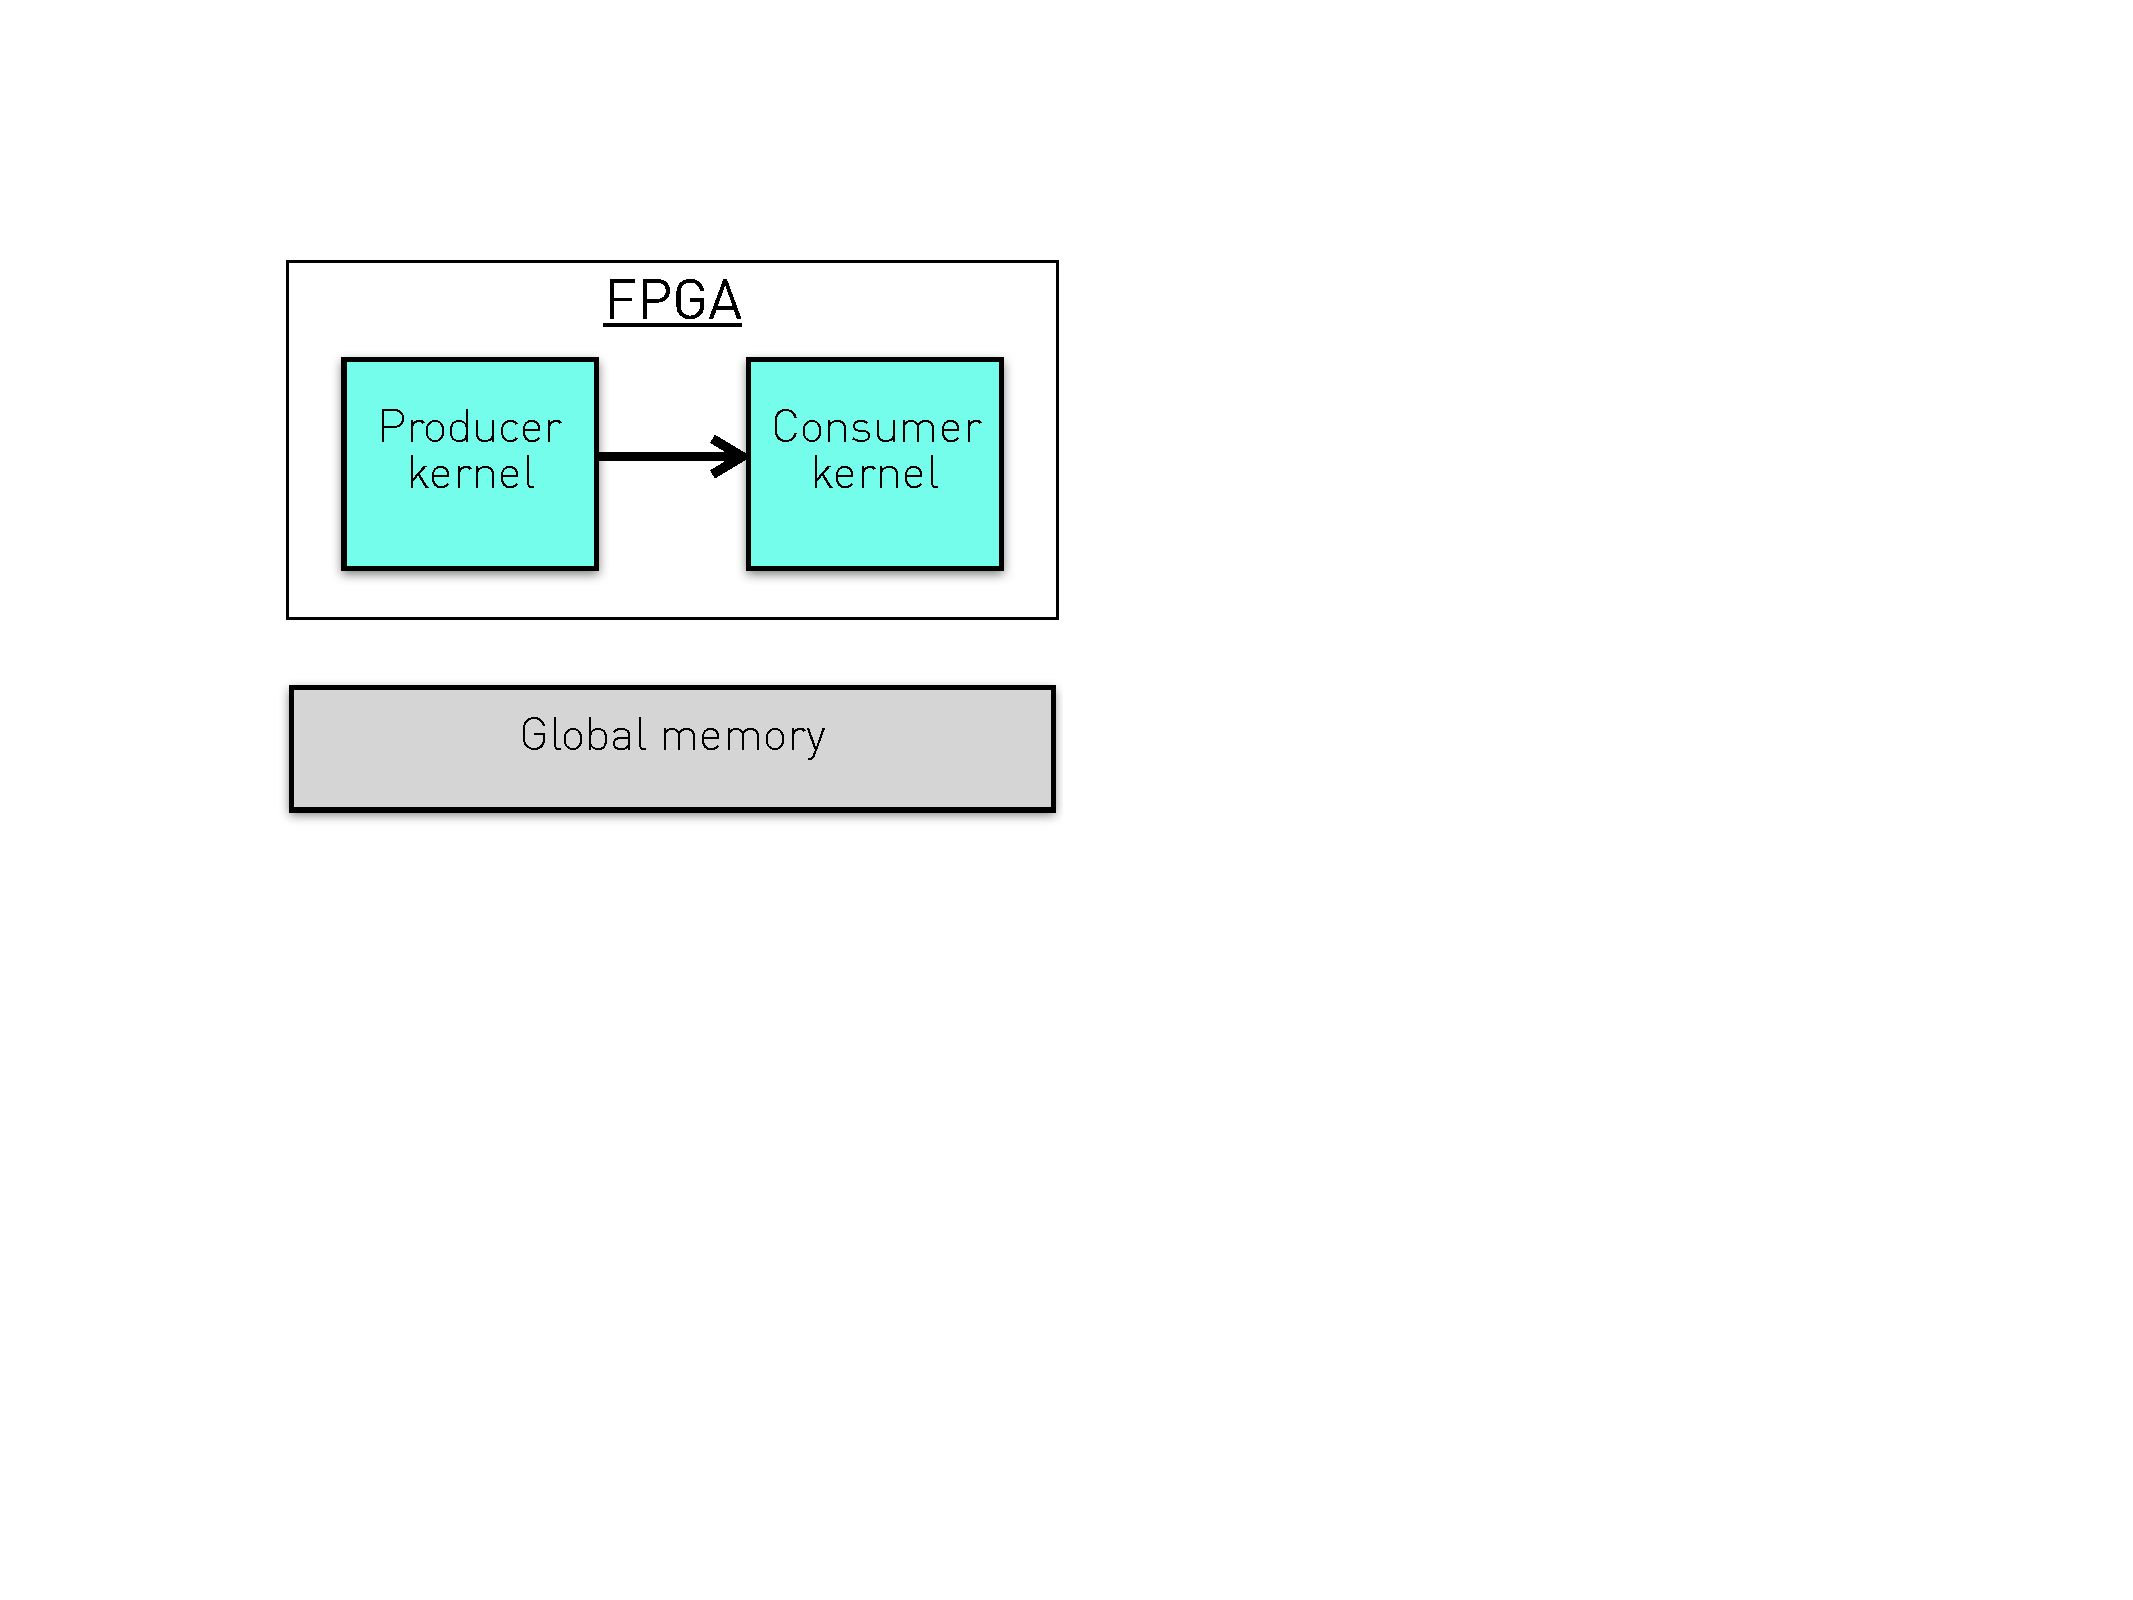
\includegraphics[width=1.4in]{with_channel.pdf} 
		\label{fig_with_channel}} % \caption{}
	\vspace{-2ex}	
	\caption{Kernel-to-kernel communication.} %: Hogwild and ModelAverage$\lambda$ is $1/2^{10}$ (``with RAW"), or $1/2^{13}$ (``without RAW"). 
	\label{fig_kkc} 
	\vspace{-2ex}
\end{figure}  



%\subsection{Dependency}
%For compute-bound applications, which can be benefited from exploring more parallelism among work items. 

\vspace{-1ex}
\section{Four OpenCL Execution Models}
\label{sec_execution_models}
%Since the architecture of FPGAs is significantly different from that of GPUs, we need to revisit the OpenCL execution models on FPGAs. with the proposed aspects in mind, 
Enabled by two go-beyond features of OpenCL on FPGAs, we identify four execution models in the context of OpenCL kernel on FPGAs. In this section, we generally analyze each execution model, in terms of programmability, computing parallelism and memory traffic. The comparison is highlighted in Table~\ref{t_comparison}.%The detailed 
%{NDRange vs. single work-item}
%{single-kernel vs. multiple kernels connected by OpenCL channel }

\begin{table} %[!hbp]
	\centering
	%\begin{spacing}{0.3}
		\begin{scriptsize}
	\begin{tabular}{|c|c|c|c|c|}
		\hline
		  & NDRange & SWI & NDRange+Channel & SWI+Channel \\
		\hline
Programmability & Moderate & High & Low & Low \\
		\hline
Computing Parallelism & Moderate & Low & High & High \\
		\hline
Memory Traffic & High & Low & Moderate & Low \\
		\hline		
	\end{tabular}
		\end{scriptsize}
	%\end{spacing}
		\caption{General comparison of four execution models}
	%\vspace{-1ex}
	\label{t_comparison}
	\vspace{-6ex}
\end{table}


\vspace{-1ex}
\subsection{NDRange}
The NDRange execution model directly employs the NDRange kernel, which is the conventional OpenCL programming mode and which is widely adopted in GPU programming. It explores a massive thread-level parallelism. The optimization methods which are used by GPUs can also apply to FPGAs, e.g., shared memory. %, memory coalescing.

{\bf Programmability. }The OpenCL programmer needs to be aware of the activity of each thread to guarantee the correct execution. Therefore, it is much more difficult than the traditional sequential programming language, e.g., C. However, there is plenty of tutorial on how to program NDRange kernel, especially for GPUs, so the programmability of NDRange execution model is moderate.

{\bf Computing Parallelism. }NDRange kernel relies on massive amount of work items to explore the parallelism from the specialized hardware generated from the NDRange kernel. Therefore, we conclude that it can achieve a high computing parallelism.  

{\bf Memory Traffic. }NDRange kernel employs the multi-pass scheme to implement the parallel algorithm, leading to potentially multiple times more memory traffic. We conclude that the requirement of memory traffic is high. 
%{\bf Cons. }It may not achieve good performance on FPGAs, whose architecture is significantly different from GPUs. Suppose it works well on FPGAs, it also works well on GPUs.
%{\bf Scope. }Without any above three issues. 

\vspace{-1ex}
\subsection{Single Work-item (SWI)}
\label{subsec_swi} 
The SWI execution model directly employs the SWI kernel, which follows a sequential programming model. %In the single work-item execution pattern, the parallelism is implicit, and the OpenCL SDK will instead determine pipelined parallelism at the compilation time based on the dependency. 
%Only one work-item is alive during the execution. 


{\bf Programmability. }Programming with SWI kernel is just like C programming. Therefore, it is relatively easy to program. We conclude that the programmability of SWI kernel is high.

{\bf Computing Parallelism. }SWI kernel relies on the off-line compiler to explore the parallelism. In order to guarantee the consistence, the compiler is always conservative, leading to a low computing parallelism.  

{\bf Memory Traffic. }SWI kernel can leverage a one-pass scheme (less memory traffic) to implement the parallel algorithm, instead of the multi-pass scheme (more memory traffic). We conclude that the SWI kernel requires a low memory traffic. 

%{\bf Pros. }Easy to write the program. 
%{\bf Cons. }
%{\bf Scope. }With Atomic or multi-pass, or both. But it works only for a simple OpenCL kernel, since it can only explore limited parallelism.

\vspace{-1ex}
\subsection{NDRange + Channel}
The NDRange + Channel execution model employs an OpenCL channel to connect two NDRange kernels such that the data communication between two kernels can be done via on-chip FIFO, rather than global memory. 

{\bf Programmability. }Besides the programming difficulty from NDRange kernel, we still need to be aware of the constraint from OpenCL Channel. In particular, the producer kernel has to produce the exact data flow which the consumer kernel wants. To make things worse, work items can execute out-of-order due to the different workload of each work item, leading to unexpected data flow from NDRange kernel. We conclude that the programmability of NDRange+Channel execution model is low.

{\bf Computing Parallelism. }
Besides the high computing parallelism from NDRange kernel, OpenCL channel allows producer/consumer kernels to execute concurrently, leading to a massive parallelism. Therefore, we conclude that it can achieve a high computing parallelism.  

{\bf Memory Traffic. }NDRange kernel requires a high memory traffic. The OpenCL channel can potentially reduce the memory traffic to a certain extent. We conclude that the NDRange + Channel execution model requires a moderate memory traffic. 

\begin{table}%[hbp]
	\centering
	\begin{scriptsize}
		\begin{tabular}{|c|c|c|c|c|c|}
			\hline
			AO & MPS & KKC & Direct prediction & Potential evolution \\		
			% the 3 pattern's name is too long
			\hline
			N & N & N & NDRange & NDRange  \\
			\hline
			Y & N & N & SWI  & SWI+Channel  \\
			\hline
			N & Y & N & SWI & SWI+Channel  \\
			\hline
			Y & Y & N & SWI & SWI+Channel  \\
			\hline
			N & N & Y & NDRange+Channel & NDRange+Channel \\
			\hline
			Y & N & Y & SWI+Channel & SWI+Channel  \\
			\hline
			N & Y & Y & SWI+Channel & SWI+Channel  \\
			\hline
			Y & Y & Y & SWI+Channel & SWI+Channel \\
			\hline
		\end{tabular}
	\end{scriptsize}
	\caption{Prediction rule}
	\label{t_pattern_to_model}
	\vspace{-6ex}
\end{table}


\vspace{-1ex}
\subsection{SWI + Channel }
The SWI + Channel execution model employs OpenCL channels to connect multiple SWI kernels such that multiple SWI kernels can work together to implement a parallel algorithm. The side effect of OpenCL channel is to relax the dependency of SWI kernel.  

{\bf Programmability. }SWI kernel has a high programmability, since its programming model is sequential. However, the OpenCL Channel incurs some constraint to guarantee the correct design. We conclude that the programmability of SWI+Channel execution model is moderate.

{\bf Computing Parallelism. }Even though the SWI kernel can achieve low computing parallelism, OpenCL channel can significantly increase the computing parallelism allows producer/consumer kernels to execute concurrently, leading to a massive parallelism. Therefore, we conclude that it can achieve a high computing parallelism.  

{\bf Memory Traffic. }SWI kernel requires a low memory traffic. The OpenCL channel might further reduce the memory traffic, so we conclude that the SWI + Channel execution model requires a low memory traffic. 



\vspace{-1ex}
\section{Bridge the Gap Between Patterns and Execution Models}%: Issue and Potential
\label{sec_bridge_gap}
In this section, we explicitly bridge the gap between three OpenCL patterns and four execution models. Typically, we can directly predict the right execution model based on three patterns (Subsection~\ref{subsec_direct_prediction}). However, there is an exception about SWI, which can only achieve low computing parallelism, indicating the further optimization potential. In particular, SWI can evolve to SWI+Channel to achieve high computing parallelism (Subsection~\ref{subsec_potential_prediction}).  

\vspace{-1ex}
\subsection{Direct Prediction}
\label{subsec_direct_prediction}
Based on whether the targeted OpenCL application has any patterns (i.e., the first three columns of Table~\ref{t_pattern_to_model}), we can directly predict the execution model, as illustrated in the ``Direct prediction" of Table~\ref{t_pattern_to_model}. Typically, the OpenCL application with AO and MPS can benefit from SWI kernel, while KKC can benefit from OpenCL channel.% indicate whether the 
\vspace{-1ex}
\subsection{Potential Evolution of SWI}
\label{subsec_potential_prediction}
In this subsection, we determine whether SWI should be evolved to SWI+Channel for higher computing parallelism, as shown in the column ``Potential evolution" of Table~\ref{t_pattern_to_model}. The evolution should satisfy two conditions. 

First, there are still enough FPGA resources remaining, as SWI+Channel, which instantiates more than one SWI kernels connected by Channel, requires significantly more FPGA resources to implement. 

Second, we present a simplified analytical model to predict the targeted SWI kernel is compute-bound or memory-bound. The evolution happens only when the SWI kernel is compute-bound. In particular, the computing time $T_{comp}$ is larger than memory time $T_{mem}$, as shown in Equation~\ref{E_overall_ineq}.
\begin{equation} \begin{scriptsize}
\label{E_overall_ineq}
\vspace{-0.5ex}
T_{comp} > T_{mem}
\vspace{-0.5ex}
\end{scriptsize} \end{equation}
The computing time $T_{comp}$ is evaluated as shown in Equation~\ref{E_comp}.
\begin{equation} \begin{scriptsize}
\label{E_comp}
\vspace{-0.5ex}
T_{comp} = \frac{LTR}{II}/\#Freq, 
\vspace{-0.5ex}
\end{scriptsize} \end{equation}
where the first part $LTR/II$ is the estimated number of cycles, equal to be the loop trip count $LTC$ divided by the initiation interval $II$. The second part $\#Freq$ is the frequency of the SWI kernel obtained from synthesis report. 
   
The memory time $T_{mem}$ is evaluated to be the number of memory traffic $MT$ divided by the memory bandwidth $\#MB$, as illustrated in Equation~\ref{E_mem}, where $\#MB$ is 18GB/s on our FPGA board.  
\begin{equation} \begin{scriptsize}
\label{E_mem}
\vspace{-0.5ex}
T_{mem} = \frac{MT}{\#MB} 
\vspace{-0.5ex}
\end{scriptsize} \end{equation}

%Direct connection + analytical model. 

\vspace{-1ex}
\section{Experiment}
\label{sec_experiment}
In this Section, we firstly present the experimental setup, secondly we conduct intensive experiment to validate our observations. 

\vspace{-1ex}
\subsection{Experimental Setup}
\label{subsec_experiment_stup}
{\bf Hardware configuration.}
We conduct our experiments on a Terasic DE5a-Net board with an Altera Arria 10 GX FPGA and 8GB 2-bank DDR3 device memory. We design our kernels using Altera OpenCL SDK version 16.1. The FPGA board is connected to the host via a x8 PCI-e 3.0 interface.
	

{\bf Workloads. }We carry out our experiment with 11 OpenCL applications, as shown in in Table~\ref{t_dataset}. 
For example, eight applications are from Chai benchmark~\cite{chang2017collaborative}, which is highly optimized for GPUs.%one application is from Rodinia~\cite{rodinia_iiswc09}.

\begin{table}%[hbp]
    \centering
        \begin{scriptsize}
    \begin{tabular}{|c|c|c|c|c|c|}
        \hline
        Application & Source & AO & MPS & KKC & Datasets \\
        \hline
        BFS & \multirow{8}{*}{Chai~\cite{chang2017collaborative}} & Y & N & N & NY, NE, UT \\
        \cline{1-1} \cline{3-6}
        RSCD &  & Y & N & Y & 2000 iterations \\
        \cline{1-1} \cline{3-6}
        TQH &  & Y & N & N & Basket \\
        \cline{1-1} \cline{3-6}
        HSTI &  & Y & N & N & 256 bins \\
        \cline{1-1} \cline{3-6}
        BS &  & N & N & N & 4*4 \\
        \cline{1-1} \cline{3-6}
        SC &  & Y & Y & N & 50\% \\
        \cline{1-1} \cline{3-6}
        PAD &  & Y & Y & N & 1000*999 \\
        \cline{1-1} \cline{3-6}
        CEDD &  & N & N & Y & Peppa, Maradona, Paw \\
        \hline
        KM & Rodinia~\cite{rodinia_iiswc09} & N & N & N & 25600 points, 8 features \\
        \hline
        MM & \multirow{2}{*}{Intel demos} & N & N & N & A: 2048*1024, B: 1024*1024 \\
        \cline{1-1} \cline{3-6}
        MS &  & N & N & N & 640*800, 2000 iterations \\
        \hline
    \end{tabular}
        \end{scriptsize}
    \caption{Experimental datasets with OpenCL patterns}
    \vspace{-5.5ex}
    \label{t_dataset}
\end{table}

{\bf Comparison Methodology. }
Our evaluations mainly validate two hypotheses. First, different execution model leads to a significant performance difference (Subsection~\ref{subsec_evaluation}). Second, we can use three OpenCL patterns to determine the right OpenCL execution model (Subsection~\ref{subsection_connection}).  

\vspace{-1ex}
\subsection{Impact of Execution Model}
\label{subsec_evaluation}
In this subsection, we mainly validate that the right execution model leads to a significant performance speedup for the OpenCL application when mapping to FPGAs. In particular, we first try our best effort\footnote{Based on our more than five years' experience in programming FPGA with OpenCL, we are pretty sure that we have already found the near-optimal optimization combination for each execution model if available. } to explore the optimization combinations for each execution model of each OpenCL application, second quantitatively compare the highest performance speedup that each execution model can achieve. 


{\bf Exploring optimization combinations. }For each OpenCL application, we explore a broad range of optimization combinations for each execution model such that its performance potential has been harvested. Due to the space limitation, we take the application RSCD as an example. 
Figure~\ref{fig_optimization_combination} shows for each combination model, the performance speedup of each optimization combination over the baseline, which is optimized GPU code. X-axis is the optimization combination under all the four execution models. We can make two observations. 
First, different execution model yields an order of magnitude performance difference. In particular, the best optimization combination under ``NDRange+Channel" can achieve 43.4X, while 2.72X for the best combination under ``SWI". 
Second, the same optimization method can yield significantly different performance speedup under different execution models. For example, loop unrolling ``UL50" under ``SWI" can only achieve 1.26X performance speedup, while 43.4X under ``NDRange+Channel".  

 
%Second, SWI typically requires less memory traffic than NDRange. 
%Third, %NDRange can typically produce more parallelism than SWI.

\begin{figure*}[t]%\textwidth
	\centering
	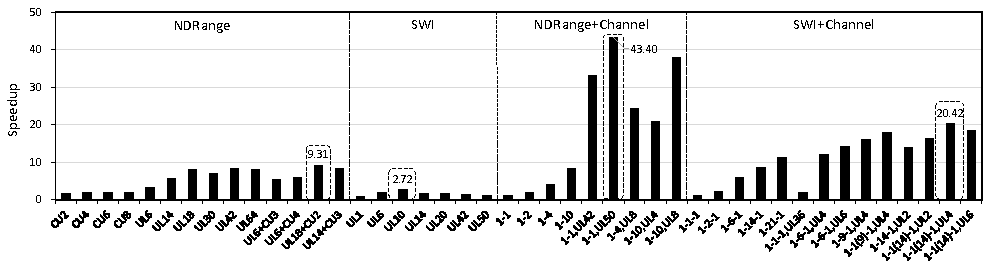
\includegraphics[width=6.05in]{rscd.pdf}
	\vspace{-3.2ex}
	\caption{Performance speedup of optimization combinations over baseline. ``CUx'' indicates x CUs, ``ULx'' indicates the loop whose unroll factor x. x-y(z)-w indicates XXX. }% We focus on the FPGA and main memory.
	\vspace{-3ex}
	\label{fig_optimization_combination}
\end{figure*} 



{\bf Speedup comparison of execution models. }
Table~\ref{t_optimization_combination} demonstrates for each execution model, the number of optimization combinations we have tried and maximum performance speedup over the baseline application which is directly imported from each source, e.g., Chai. 
We can make two observations. First, different execution model indeed results in significant performance speedup difference. Take HSTI as an example, the right execution model (SWI+Channel) can have 19.54X performance speedup over the baseline which is the optimized GPU code, while the inappropriate execution model (SWI) can only achieve 1.01X speedup. Second, different OpenCL application requires different execution model to achieve the best performance. For example, the best execution model for BFS is SWI+Channel, while NDRange is most suitable for MM. We conclude that it is critical to decide the right execution model when optimizing OpenCL application on FPGAs.  

%\begin{table}%[hbp]
%	\centering
%	\begin{scriptsize}
%		\begin{tabular}{|c|c|c|c|c|}
%			\hline
%			Application & NDRange & SWI & NDRange+Channel & SWI+Channel  \\
%			
%			
%			\hline
%			KM & 114.86 & 2.73 & 136.41 & 28.96 \\
%			\hline
%			BFS & 1.6 & 2.77 & 1.19 & 2.94 \\ 
%			\hline
%			RSCD & 9.31 & 2.72 & 43.4 & 20.42 \\
%			\hline
%			TQH & 1 & 1.28 & & 2.98 \\
%			\hline
%			HSTI & 2.67 & 1.06 & 9.49 & 19.54 \\
%			\hline
%			BS & 3.01 & 10.77 & 3.34 & 44.06 \\
%			\hline
%			SC & 1.52 & 4.51 &  & 17.13 \\
%			\hline
%			PAD & 1 & 1.6 &  & 4.8 \\
%			\hline
%			CEDD & 2.95 & 0.02 & 2.72 & 0.03 \\
%			\hline
%			MM & 837.12 & 0.73 & & 0.72 \\
%			\hline
%			Mandelbrot & 34.72 & 2.48 & & 3.17  \\
%			
%			\hline
%		\end{tabular}
%	\end{scriptsize}
%	\caption{Optimization combinations: number and speedup }
%	\label{t_optimization_combination}
%\end{table}


\begin{table}%[hbp]
	\centering
	\begin{scriptsize}
		\begin{tabular}{|c|c|c|c|c|c|c|c|c|}
			\hline
		    \multirow{2}{*}{Application} & \multicolumn{4}{c|}{Number of combinations} & \multicolumn{4}{c|}{Maximum speedup} \\
         \cline{2-9}
			
			 %& NDRange & SWI & NDRange+Channel & SWI+Channel & NDRange & SWI & NDRange+Channel & SWI+Channel \\
			& NDR & SWI & NDR+C & SWI+C & NDR & SWI & NDR+C & SWI+C \\
			
			\hline
			KM & 30 & 14 & 12 & 17 & 147.67 & 8.76 & 136.41 & 28.96 \\
			\hline
			BFS & 17 & 1 & 1 & 4 
			& 1.85 & 2.95 & 1.22 & 2.96 \\ 
			\hline
			RSCD & 22 & 10 & 24 & 39 & 9.31 & 2.72 & 43.4 & 20.42 \\
			\hline
			TQH & 1 & 15 & & 20 & 1 & 1.28 & & 2.98 \\
			\hline
			HSTI & 9 & 36 & 9 & 28 & 2.67 & 1.06 & 9.49 & 19.71 \\
			\hline
			BS & 20 & 17 & 18 & 8 & 3.01 & 10.77 & 3.34 & 44.06 \\
			\hline
			SC & 15 & 34 & & 9 & 1.52 & 4.51 &  & 17.13 \\
			\hline
			PAD & 11 & 10 && 14 & 1.15 & 1.6 &  & 4.8 \\
			\hline
			CEDD & 55 & 9 & 25 & 2 & 2.95 & 0.01 & 2.72 & 0.02 \\
			\hline
			MM & 25 & 3 && 1 & 837.12 & 0.73 & & 0.72 \\
			\hline
			MS & 7 & 6 && 7 & 34.72 & 0.02 & & 3.17  \\
			
			\hline
		\end{tabular}
	\end{scriptsize}
	\caption{Space exploration of optimization combinations }
	\label{t_optimization_combination}
	\vspace{-5ex}
\end{table}





 

%Hypotheses to validate:Evaluation of 

\vspace{-1ex}
\subsection{Prediction of Right Execution Model}
\label{subsection_connection}
In this subsection, we mainly validate that for each OpenCL application, the prediction of execution model matches the empirical result. Essentially, we can predict the right execution model, which can produce best performance, based on three OpenCL patterns (Section~\ref{sec_bridge_gap}). Table~\ref{t_prediction_execution_model} shows the predicted execution model, as well as the real execution model which can achieve the best performance in our real experiment. 
We can observe that the prediction of execution model almost matches the real experimental result.    
%Second, .



\begin{table}%[hbp]
	\centering
	\begin{scriptsize}
		\begin{tabular}{|c|c|c|c|c|c|}
			\hline
			Application & AO & MPS & KKC & Real & Prediction\\
			
			% the 3 pattern's name is too long
			
			\hline
			BFS & Y & N & N & SWI+Channel & SWI+Channel  \\
			\hline
			RSCD & Y & N & Y & NDRange+Channel & SWI+Channel \\
			\hline
			TQH & Y & N & N & SWI+Channel & SWI+Channel \\
			\hline
			HSTI & Y & N & N & SWI+Channel & SWI+Channel \\
			\hline
			BS & N & N & N & SWI+Channel & NDRange \\
			\hline
			SC & Y & Y & N & SWI+Channel & SWI+Channel \\
			\hline
			PAD & Y & Y & N & SWI+Channel & SWI+Channel \\
			\hline
			CEDD & N & N & Y & NDRange & NDRange+Channel \\
			\hline
			KM & N & N & N & NDRange & NDRange \\
			\hline
			MM & N & N & N & NDRange & NDRange \\
			\hline
			MS & N & N & N & NDRange & NDRange \\
			\hline
		\end{tabular}
	\end{scriptsize}
	\caption{Prediction of execution model}
	\label{t_prediction_execution_model}
	\vspace{-5ex}	
\end{table}




\vspace{-1ex}
\section{Conclusion}
Despite the preliminary success of programming FPGA with OpenCL, direct adoption of OpenCL cannot fully harvest the performance potential of FPGAs, since the architecture of FPGAs is significantly different from that of GPUs, for which OpenCL is originally designed. In particular, the OpenCL programmer should be aware of two go-beyond OpenCL features to explore the performance potential of FPGAs. However, the OpenCL programmer still requires an end-to-end guideline about how to leverage these two features. In this paper, we bridge the gap between three typical OpenCL patterns and four execution models (aware of go-beyond OpenCL features). Experimental result shows that the right execution model can yield three order of magnitude performance difference. 

\noindent
{\bf Acknowledgement. }We thank Intel which has generously donated Terasic\textquoteright s DE5A-Net Arria 10 FPGA board for our research.   
%2, The necessary background of FPGA is required to guarantee the good performance of OpenCL kernels on FPGAs. 
%3, for the beginner, OpenCL is much easier than RTL . 

%Two observations are orthogonal. 

%1, Multi-pass and atomic operations can benefit from single-work item.

%2, Multiple kernels (producer-consumer) can benefit from channel. 

%3, NDRange can explore more pipelined parallelism than single-work-item. (Using one example (MM) to show).




\vspace{-1ex}

%We thank Altera and Intel for hardware donations. This work is supported by a MoE AcRF Tier 1 grant (MOE 2014-T1-001-145), an NUS startup grant and a HKUST startup grant (R9336).

%This work is in part supported by MoE AcRF Tier 2 grants (MOE2012-T2-1-126 and MOE2012-T2-2-067) in Singapore.
%\vspace{-2ex}

\bibliographystyle{abbrv} %ACM-Reference-Format}
%\linespread{.2}
%	\scriptsize
\bibliography{myref}



\end{document}
